\subsubsection{\stid{3.02} The Flexible Computational Science Infrastructure (FleCSI) Project} 

\paragraph{Overview} 

FleCSI\cite{FleCSI} is a compile-time configurable framework designed to
support multi-physics application development. As such, FleCSI attempts
to provide a very general set of infrastructure design patterns that can
be specialized and extended to suit the needs of a broad variety of
solver and data requirements. Current support includes multi-dimensional
mesh topology, mesh geometry, and mesh adjacency information,
n-dimensional hashed-tree data structures, graph partitioning
interfaces, and dependency closures, e.g., to identify data dependencies
between distributed-memory address spaces.

FleCSI also introduces a functional programming model with control,
execution, and data abstractions that are consistent with state-of-the-art
task-based runtimes such as Legion\cite{Bauer:2012:LEL:2388996.2389086}
and Charm++\cite{Kale:1993:CPC:165854.165874,
Kale:1993:CPC:167962.165874}.  The FleCSI abstraction layer provides the
developer with insulation from the underlying runtime, while allowing
support for multiple runtime systems, including conventional models like
asynchronous MPI\cite{TheMPIForum:1993:MMP:169627.169855}.  The intent
is to give developers a concrete set of user-friendly programming tools
that can be used now, while allowing flexibility in choosing runtime
implementations and optimizations that can be applied to architectures
and runtimes that arise in the future.

FleCSI uses static polymorphism, template meta-programming techniques,
and other modern C++ features to achieve high runtime performance,
customizability, and to enable DSL-like features in our programming
model. The FleCSI program structure adopts a three-tiered approach: a
low-level core library that is specialized by a mid-level layer to
create high-level application interfaces that hide the complexity of the
underlying templated classes. This structure facilitates separation of
concerns, both between developer roles, and between the structural
components that make up a FleCSI-based application.

As an example of how this works in practice, consider the FleCSI mesh
topology type:

The low-level mesh interface is parameterized by a policy, which defines
various properties such as mesh dimension, and concrete entity classes
corresponding to each topological domain and dimension. The mesh policy
defines a series of tuples in order to declare its entity types for each
topological dimension and domain, and select connectivities between each
entity. FleCSI supports a specialized type of localized connectivity
called a {\it binding}, which connects entities from one domain to
another domain.

FleCSI separates mesh topology from geometry, and the mesh--from the
topology's perspective--is simply a connected graph. Vertex coordinates
and other application data are part of the {\it state model}. Our
connectivity computation algorithms are based on
DOLFIN\cite{Logg:2010:DAF:1731022.1731030}.  Once vertices and cells
have been created, the remainder of the connectivity data is computed
automatically by the mesh topology through the following three
algorithms: {\it build}, {\it transpose}, and {\it intersect}, e.g.,
{\it build} is used to compute edges using cell-to-vertex connectivity
and is also responsible for creating entity objects associated with
these edges. From a connectivity involving topological dimensions
$D_1 \rightarrow D_2$, transpose creates connectivity $D_2 \rightarrow D_1$.
Intersect, given $D_1 \rightarrow D'$ and $D' \rightarrow D_2$, computes
$D_1 \rightarrow D_2$.  

The low-level mesh topology provides a set of iterable objects that a
mid-level specialization can make available to an application to allow,
at a high-level, iteration through connectivities using an intuitive
{\it ranged-based for} syntax, e.g., forall cells $c_i$, forall edges
$e_i$ of cell $c_i$. Entities can be stored in sets that also support
range-based for iterations and enable set operations such as union,
intersection, difference, and provide functional model capabilities with
{\it filter}, {\it apply}, {\it map}, {\it reduce}, etc.

\paragraph{Key Challenges}

As part of the LANL ATDM effort, FleCSI is one component in a rapidly
shifting environment of new software and simulation approaches. This
poses several challenges. In particular, the fast evolution of both the
runtime backends used by FleCSI, and the applications that are built on
top of it make development of FleCSI itself a challenge. Because FleCSI
is the fulcrum of a complicated co-design process, it is exposed to
instabilities and design challenges from above and below.

FleCSI also faces the challenge of developing a programming model that
can span the diverse set of system and node-level architectures for
planned and current DOE procurements. Although there is a consistent
theme of increased parallelism and scale, the details of individual
processor and accelerator architectures present subtly different models
of fine-grained parallelism that prove challenging to abstract.

Finally, FleCSI is also seeking to develop fundamental data structures
and abstractions that will enable a new and sustainable development
process that also satisfies the scope of the LANL ATDM project. This
requires careful investigation of requirements and interface design that
are essentially collaborative, and reach across institutional and
cultural barriers within our organization. These relationships are often
challenging to negotiate, and require maturity and a broad knowledge
base.

\paragraph{Solution Strategy}


Our general strategy is one of communication and co-design, whereby, we
work in carefully constructed, multi-disciplinary teams to identify
gaps in the FleCSI model, design and implement abstractions to fill
these gaps, and then verify them in compact applications. To address
the challenge of operating in a fluid design environment, we often
freeze several components of the application and/or backend runtime to
isolate a particular area for refactoring or enhancement. This approach
requires a modular design, which is one of the cornerstones of the
FleCSI project, and one that has been successfully exercised in several
instances.

\paragraph{Recent Progress}

Recent progress on the FleCSI project has seen the addition of several
new storage classes for representing unstructured and sparse data. In
particular, we have added \textit{sparse} and \textit{ragged} storage
classes. The sparse storage class provides an interface to logically
sparse data, e.g., that might arise in the representation of
multi-material models or sparse matrices. The ragged storage type is
similar, but does not have the notion of columnar indices. Both of these
storage types allow dynamic resizing and mutability of the sparsity
structure of the represented data. Additionally, we have added
\textit{global} and \textit{color} storage classes that allow the
representation of simulation state that is either a singleton, or that
is on a per-color (the task version of an MPI rank) basis, respectively.

Other recent enhancements include a simplified and improved
interoperability interface for managing and interacting with MPI tasks,
an improved futures interface, and C++ language extensions for
fine-grained data parallel operations.

\paragraph{Next Steps}

Current work includes performance testing and tuning. Modifications 
to enable compilation with Kitsune compiler from MIT. Additional 
features to support checkpoint-restart, changes to support formated 
input, geometeries and mesh models and allow applications to be driven 
from existing Common-Model infrastructure.
%Future work will include the design and implementation of a
%\textit{set topology} data structure that is suitable for representing
%several different classes of particles, e.g., \textit{particle-in-cell
%(PIC)} method, \textit{material-point method (MPM)}, and
%\textit{Monte Carlo (MC)} methods. We are also working to incorporate
%changes to the Legion programming model that will provide: a more formal
%interface for reasoning about and managing graph coloring
%\textit{dependent partitioning}, and an improved task model that will
%significantly increase scalability \textit{control replication}.
%Control replication is an important design improvement to Legion, as it
%will allow runtime management of dynamically changing data types in a
%more efficient manner than is currently possible. We will continue to
%engage in co-design with runtime and application developers to refine
%and improve the FleCSI model and interface.

\begin{figure}
  \centering
  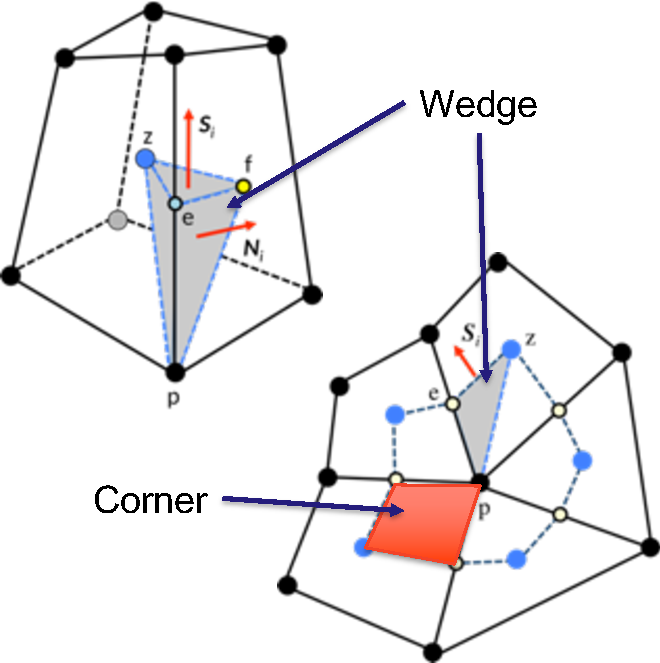
\includegraphics[scale=0.6]{projects/2.3.3-MathLibs/2.3.3.02-LANL-ATDM-MathLibs/mesh.pdf}
  \caption{FleCSI unstructured mesh example from the FleCSALE application.}
  \label{fig:mesh}
\end{figure}
